\documentclass[paper=a4,fontsize=12pt]{scrartcl}
\usepackage{geometry}
\usepackage{graphicx}
\geometry{verbose, a4paper, tmargin=25mm, bmargin=25mm, lmargin=25mm, rmargin=25mm}

\usepackage[utf8]{inputenc}
\usepackage[ngerman]{babel}
\usepackage{fancyhdr} %Paket laden
\pagestyle{fancy} %eigener Seitenstil
\fancyhf{} %alle Kopf- und Fußzeilenfelder bereinigen
\fancyhead[L]{
\includegraphics[width=3cm]{img/logo_bfh_de.jpg}} %Kopfzeile links
\fancyhead[C]{} %zentrierte Kopfzeile
\fancyhead[R]{Janosch Rohdewald, Marco Füllemann} %Kopfzeile rechts
\renewcommand{\headrulewidth}{0.4pt} %obere Trennlinie
\fancyfoot[C]{\thepage} %Seitennummer
\renewcommand{\footrulewidth}{0.4pt} %untere Trennlinie

\begin{document}
\section*{Walter mit Matlab suchen}
\subsection*{Konzept}
Wer kennt die Kinderbuchreihe ``Wo ist Walter?'' nicht? Auf den Bildern sind jeweils hunderte von Menschen zu sehen, zum Beispiel Stadtszenen, Jahrmärkte oder überfüllte Strände. Walter ist immer mit einer Brille, einem rot-weiß gestreiften Pullover und einer Pudelmütze bekleidet. Dabei ist zu erwähnen, dass um das Finden von Walter zu erschweren die Umgebung von Walter ziemlich chaotisch ist, und Ähnlichkeiten mit ihm aufweist. 
\begin{figure}[htbp] 
  \centering
     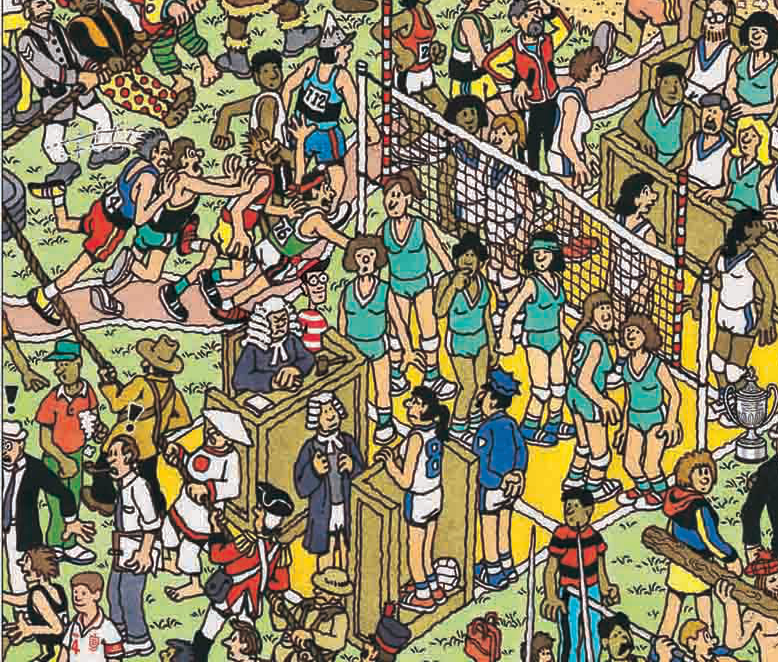
\includegraphics[width=0.7\textwidth]{img/Wally.png}
  \caption{``Wo ist Walter?'' Im Wembley Stadion (Ausschnitt)}
  \label{fig:Bild1}
\end{figure}

In dieser Arbeit wollen wir durch die Verwendung von Computer-Perception-Algorithmen Walter mit Matlab finden. Dabei wird ein Ansatz nicht ausreichen, sondern es müssen mehrere kombiniert werden.
\begin{itemize}
 \item Extrahieren der Farben rot und weiss um mögliche Pullover zu finden
 \item Mögliche Brillen mittels Hough Transformation identifizieren
 \item Farbe des Gesichts filtern
\end{itemize}
Aus jedem dieser Ansätze wird es mehrere Mögliche Orte geben, wo Walter sein könnte. Wird der Output jedoch korreliert sollte es nur noch ein Rechteck bestimmter Grösse (Walter) geben, wo sich Walter verstecken kann. 


\section*{Erwartete Resultate}

\end{document}